\documentclass[a4paper,12pt]{article}

\usepackage{rotating}
\usepackage[top=1in, bottom=1in, left=1in, right=1in]{geometry}
\usepackage{graphicx}
\usepackage[numbers,square,sort&compress]{natbib}
\usepackage{setspace}
\usepackage[cdot,mediumqspace,]{SIunits}
\usepackage{caption}
\usepackage{subcaption}

\begin{document}
\onehalfspacing
\title{Final report of a CTA399 student's work with VLBI pulsar observations}
\author{Natalie Price-Jones}
\date{30 August, 2013}
\maketitle

%%%%%%%%%%%%%%
\begin{abstract}
\label{abstract}


Pulsars, periodic radio sources, emit radiation in characteristic pulses that vary in shape and frequency. The mechanism whereby such pulses are generated is still not well understood, but with greater resolving power it might prove possible to probe the nature of the pulses in more detail. This may lead to the discovery of the intricacies of the magnetic field that produces such striking lighthouse emission. To achieve the requisite level of resolving power, this project aims to use Very Long Baseline Interferometry (VLBI) to resolve the images of the pulsar that have been scattered by interstellar medium. Such scattering provides an opportunity for interferometry with a baseline on the order of an astronomical unit, further resolving the pulsar to nanoarcsecond precision. To this end, raw voltage observations were taken at \unit{325}{\mega\hertz} and \unit{150}{\mega\hertz} on bright calibrator sources and fainter millisecond pulsars at the ARO, GMRT, LOFAR and Effelsberg telescopes.  In order to constructively add the signal from the different locations, it was necessary to shift them into the same phase. Increasing the signal to noise ratio on the relatively faint pulsar was also essential. We have successfully spotted both bright and millisecond pulsars at ARO and GMRT. At the moment, the project is still in the early stage of interpreting observations, confirming pulsar sightings at each individual telescope, and further observations will be taken later in the year in order to attempt the interstellar interferometry that is the primary aim. 

\end{abstract}

%%%%%%%%%%%%%%
\section{Introduction}
\label{sec:introduction}

\subsection{Pulsars}
\label{sec:pulsars}

Pulsars, by emitting in radio at well-defined intervals, provide a useful observational source with a known timescale. This property of periodic emission is helpful because a pulsar is either 'on' or 'off', and the shifts between these two states make it obvious against the continuum of the background. In addition, pulsars are point sources, unaffected by the smearing that distorts larger objects. Their point source nature also allows for observable scintillation. 

All stellar objects visible to the naked eye can be seen to scintillate. The term refers to the 'twinkling' caused by turbulence in the Earth's atmosphere where stars seem to grow brighter and fainter with time. Pulsars exhibit the same phenomenon, though it is invisible to the unassisted human observer - as is the pulsar itself in all but a few cases. Like the earth's atmosphere, the clumps of gas and dust that make up the interstellar medium (ISM) cause scintillation in radio sources. The scintillation has a timescale anywhere from hours to days (source) - much longer than the period of any pulsar. There is not yet an agreed upon model that explains the various properties of this pulsar signal scattering. Unlike the twinkling of stars, pulsar scintillation is not the product of turbulence. Turbulence is a random process, and that random quality would be evident in observations. Instead, images of the pulsar caused by its lensing through the ISM are clearly distributed along a line. In addition, a turbulent scattering model would require overdensities in the ISM much higher than can be easily accounted for by known plasma behaviors. From this, it has been proposed that the pulsar's regular signal (the pulse), has been scattered by a thin sheet, the exact geometry of which has yet to be determined (Walker et al).

For the purposes of this project, the exact mechanism of pulsar scintellation is not as import as the property itself. A new technique, dubbed scintellometry, makes use of it in an interesting way.


\subsection{Scintellometry and VLBI}
\label{sec:scintellometry}

Very Long Baseline Interferometry (VLBI), is a technique used by radio astronomers to extend the baseline of their observations and thus gain greater resolving power. Any two telescopes that can see the same source in the sky can be used to perform interferometry. Since the distance between telescopes is known and it is possible to calculate the difference in signal arrival time between them. With this information, the signal can be phased up - that is, the data is shifted so that the signal from each telescope is added up in phase. This can be done on small scales (as with GMRT's 30 antennas), as well as very large ones. In the case of VLBI, the distances are akin the diameter of the planet – as if the entire Earth were a single huge dish. The larger the distance between the two receivers of the signal, the greater the resolving accuracy, since the diffraction limit is inversely proportional to the diameter of the receiving dish. Current VLBI achieves an angular resolution on the order of milliarcseconds. 

However, scintellometry makes use of pulsar scattering to decrease the diffraction limit exponentially - down to the nanoarcsecond scale. This will be done by using the ISM itself as a series of antennas with a baseline of an astronomical unit. To do this, VLBI will be done with several telescopes across the world. These telescopes will be used to resolve the images of the pulsar scattered by the ISM. By applying the components of interferometry again on a grander scale, it will be possible to treat the scattered images as the signal reaching an array of telescopes with a baseline the size of Earth's orbital radius.

This new technique would make it possible to probe the nature of pulsars more deeply than before, perhaps even affording some understanding of the ways in which they produce pulses. Even with the greater resolution afforded by scintellometry, it would not be possible to actually discern the actual shape of even the closest pulsars. However, greater resolution would allow development of theories of the reason for pulsars' unusual emission.

\subsection{Why Radio?}
\label{sec:radio}

Observing in radio has a few advantages over its optical counterpart. While most Earthbound astronomy is hampered by the fluctuations and molecular absorption in the atmosphere, this does not pose a problem for radio astronomers. They are forced to contend with emission rather than absorption. Radio astronomy also means that VLBI is possible - an essential feature of the current project. Observing in radio wavelengths ensures that pulse signals are actually scattered, where a wave with a shorter wavelength might pass through unscathed.

\subsection{Goals}
\label{sec:goals}

The overall aim of this project is to use VLBI to perform scintellometry and increase the resolution on pulsar targets of scientific interest. This summer’s work was a step in that direction. First, the software needed to be tested, then the VLBI itself was done at two different wavelengths. Before it is possible to contemplate scintellometry, it will be necessary to see the pulsar at each of the telescopes that will ultimately be used. Observations taken this summer will be used to that end.

%%%%%%%%%%%%%%

\section{Observations}
\label{observations}
The highlights of the course were the two trips made to ARO to do VLBI work, but many observations were made over the course of the summer.

\subsection{Tests}
\label{tests}
The tests were conducted entirely at GMRT, and for the most part involved software adjustments. A new bandwidth option was developed for the raw voltage GMRT data correlator - \unit{32}{\mega\hertz} in place of the usual 16. This required some trial runs before bringing it to bear on VLBI. Test observations were run on May 16, June 11 and June 29. The first two were conducted at \unit{325}{\mega\hertz}, the third at \unit{150}{\mega\hertz}. My part in the observations was limited to communicating with the GMRT operator - relaying our intended plan for our alotted time and the settings we wanted to test as well as ensuring things stayed on track as the test progressed. It was during one of these tests that we discovered the importance of double checking the LO frequency that would be used to mix the signal down. During the June 29 observations, we decided on the importance of a system that would name files based on a timestamp rather than relying on the name being changed manually. 

We observed a variety of targets, including pulsar B1919+21, millisecond pulsar B1957+20, and the crab pulsar. The former two would be targets of the VLBI observations, and data taken over a separation weeks might offer some evidence of scintillation that might not be glimpsed on the shorter timescale of individual observations.

\subsection{VLBI}
\label{vlbi}

Two week-long trips were made to ARO, one on June 24 (observing frequency: \unit{325}{\mega\hertz}) and the other on July 21 (observing frequecy:\unit{150}{\mega\hertz}). Both instances of VLBI included ARO and GMRT, with Effelsberg providing more baselines in the former case and the aptly named LOFAR in the latter. Targets were reasonably consistent: bright pulsars with period on the order of a second like B1919+21, B2111+46, and B0329+54, as well as fainter millisecond pulsars like B1957+20, and J1810+1744.

\section{CITA Computing}
\label{sec:CITAcomputing}

At the beginning of my involvement with this project, the Canadian Theoretical Institute of Astrophysics (CITA) computing environment was a complete unknown to me. As such, it was necessary to come to grips with a few essential tools to become proficient at CITA computing.

\subsection{Git Repositories}
\label{sec:git}

For this project, git repositories were the primary location of necessary code. The general repository was mhvk/scintellometry.git. This repository contained code for gathering and analyzing pulsar data from all four telescopes used in the project. Anyone working on the project could create their copy of the scintellometry git repository and make changes to files they wanted to work with. Requests would be sent to merge these changes if they were deemed useful for everyone involved.

An additional repository, NatalieP-J/work-share.git tracked progress on my individual assignments. The repository was created to more easily share files between home and work machines, so that the working version of a particular code would always be the most up to date in either location. The repository also contains many supplementary files, including timestamp files, generated delay times, generated sequence files and journal articles.

The commented versions of unique codes I wrote are located in this repository in the Code directory. A subdirectory called Edits contains the code I needed to change to use.

\subsection{Package Set Up}
\label{sec:packagesetup}

Computing at CITA starts with a desktop machine, but other, faster machines are readily available, some with different software configurations. For this project, where a good Python environment was important, chime and prawn were used often. A desktop machine at CITA often raised problems when running Fortran90 code, and such issues were not present on the faster machines.

Python was the language of choice for my assignments, and so it was necessary to build a proper environment within my CITA account. In particular, installing up to date versions of numpy, matplotlib and novas for python as well as the latest developer build of astropy was essential. It is these four packages upon which most of the python code was based. Other modules used were generally built in ones for the Python 2.7.5. It was this version of Python that was kept as standard for Python code written this summer.

\subsection{SSH Keys}
\label{sec:sshkeys}

The final useful component of CITA computing also extended to other systems – SSH keys. These proved invaluable for remote access of CITA from my home machine as well as working across multiple machines at GMRT.

\section{Giant Metrewave Radio Telescope Computing}
\label{sec:gmrtcomputing}

The Giant Metrewave Radio Telescope (GMRT) setup of computers can be accessed remotes with the correct passwords to get through a gateway machine. I was given access to nodes 17-48 and nodes 111-118 to work on, as well as the root password. This gave me the ability to mount disks from each node as was necessary. Each node at GMRT has four disks mounted on it, each of these disks with multiple partitions. The raw dump voltage software backend records information to sixteen nodes at a time, to each of the four disks simultaneously. This takes up quite space quickly, and because of this, most of the work that needed to be done at GMRT was of a data crunching variety.

\subsection{Python at GMRT}
\label{sec:pythonatgmrt}

In order to run Python scripts at GMRT, it was necessary to install an updated version of Python. The chosen distribution was Anaconda. This initially some problems with library locations for other codes, but was resolved by editing the shell login file. The distribution was installed in the /mnt/code directory, which is mounted across all nodes – an important factor when trying to run a script across a sequence of nodes.

\subsection{Disk Mounting}
\label{sec:diskmount}

One particular assignment involved copying data from the nodes 17-32 cluster to the nodes 33-48 cluster (hereafter referred to as the old and new cluster respectively). The data to be moved was taken during the second VLBI run this summer, from July 21 to July 28. The script read from four disks on the old cluster and copied the data to four disks on the new cluster, which made the process much faster than secure copying each file individually. However, the script also required consistent naming of the disks to be written to. It was necessary that disks with enough space to hold the files be mounted on a node of the new cluster and given a consistent naming scheme. This work was largely done manually during overnight copying sessions, since disk space fluctuated over the course of the week and had to be recounted every night.

In addition to this, some of the disks were unmounted during reboots, causing us to believe there was less space available than there actually was. From time to time, even the essential disks were unmounted so that files went missing. Fortunately, existing scripts allowed us to efficiently remount the disks on both clusters (once the scripts were located).

\subsection{Fringestopping}
\label{sec:fringestopping}

Another assignment was fringestopping, a data reduction routine that was hoping to clear out some space on the nodes 111-118 cluster. A description of the details of the process can be found on this project's wiki. This process ran smoothly for some January 2013 data fringestopped for Liam Connor, but required more thought for older data belonging to Prasun Dutta. The main concern was missing files and poor file locations. Dutta’s files had been transferred from the 33-48 cluster of nodes in suboptimal manner, and it was necessary write a script to locate all the requisite files to run the program. Dutta also required a higher number of frequency channels, and it took quite a while to confirm that the fringestop was still doing what was expected of it (see Figure~\ref{fig:failedFS} for unexpected results). This was checked by examining lag plots of the data in search of a pulsar. In the end, the fringestop was successful for scans where enough files could be found for it to run (see Figure~\ref{fig:successfulFS} for the aimed for results). However, with over 900 of Dutta’s scans to process, no significant headway was made before the end of the summer.

The code used to locate and link together the files for fringestopping is located within the Code directory mentioned in section~\ref{sec:git}

\begin{figure}
\centering
\begin{subfigure}{0.5\textwidth}
  \centering
  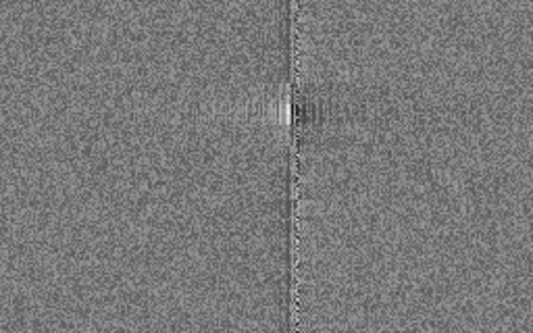
\includegraphics[width=\linewidth]{256ChanLag.pdf}
  \caption{A successful fringestop of Dutta's data using 128 frequency channels. The bright spot is the pulsar.}
  \label{fig:sub1}
\end{subfigure}%
\begin{subfigure}{0.5\textwidth}
  \centering
  
\includegraphics[width=0.8\linewidth]{4096ChanFailedLag.pdf}
  \caption{An example of a possible unsuccessful fringestop lag using 2048 frequency channels. The data is garbled and the pulsar is not visible.}
  \label{fig:sub2}
\end{subfigure}
\caption{Unsuccessful or undesired fringestopping results on the sixth scan taken on pulsar B0329+54 on August 22 2012 by Prasun Dutta.}
\label{fig:failedFS}
\end{figure}

\begin{figure}
\centering

\includegraphics[width=\linewidth]{4096ChanLag.pdf}

\includegraphics[width=\linewidth]{lag102.pdf}
\caption{The results of a successful fringestop using 2048 frequency channels on the same scan used in Figure~\ref{fig:failedFS}. The top image is a cropped section of bottom one, zoomed to show the pulsar. In the original image, the pulsar is just visible as a white dot in the center. This original image is the exact product of the process used to generate Figure~\ref{fig:sub1} and has a far higher resolution of the pulsar image.}
\label{fig:successfulFS}
\end{figure}

\subsection{Epoch of Reionization Project}
\label{sec:eor}

Another project worked on was monitoring the Epoch of Reionization (EoR) correlator. This was another space juggling exercise on nodes 33-48. The data was written to the disk called EoR\_correlation on each node, but space was consumed at a ferocious rate. My monitoring duties consisted mostly of ensuring enough space remained on each such disk. This required using a few python scripts to investigate the disk situation.

\section{Algonquin Radio Observatory}
\label{sec:aro}

Work at ARO was more varied in that it was not uniformly software based. As at GMRT, the ARO setup had a variety of nodes (5, in this case, with a few backups and spares). In total, there are three versions of the ARO setup that I am aware of  - two at CITA for testing as well as the one actually in use at ARO.

\subsection{Hardware}
\label{sec:hardware}

For each ARO setup created, it was necessary to install the correct CenTOS 6 as well as a number of libraries. In addition, two of the nodes need to Analog to Digital Converter (ADC) boards. We installed these in the nodes at ARO, and moved the board when one of the nodes needed to be swapped out. We also installed large hard drives in each node to maintain the high rate of data acquisition.

In addition, we helped with feed construction by building a ground plane and the smaller fat dipole antenna modeled after GMRT’s antennas. However, both of these were eventually deconstructed in favor of the final product.

\subsection{Ubuntu Node (Pen Node 10)}
\label{sec:ubuntunode}

In addition to the four nodes used for acquisition and processing of the data, there was a fifth running a 64bit operating system (OS) that gave us a real time display of the signal hitting the feed. I set up this node with some assistance from Phil Isaac with the operating system. Though it was a 64bit OS, it needed 32bit libraries to work with the other nodes.  I installed Python and the primarily used modules and set up at git account for the machine which wouldn’t be tied to any particular user. In addition, I copied over the 32bit openmpi and intel libraries from the CITA network as well as installing a newer, 64bit version of openmpi.

\section{Pulsar Folding}
\label{sec:pulsarfolding}

Pulsar folding is the process of binning time and adding across a pulsar’s period so that signal of the pulse is increased while the surrounding noise is decreased. If folding from multiple antennas, it is also necessary to account for the delays between them. Adding up a signal from multiple antennas (phasing) also increases the signal to noise, as well as the resolution.

\subsection{Delay Times}
\label{sec:delaytimes}

In order to phase together the signal at each GMRT antenna (as well as the different VLBI locations), it was necessary to generate delay files. Such files consisted of the delay in metres for each location of interest for each timestamp during an observation.

At first, the files were generated with many small codes in languages including Fortran90, C, Perl, and Python. After the first VLBI run of observations, a Python script was written that incorporated all of these steps into a single, stream-lined process. Key points in the process were finding the location of the antennas in the appropriate coordinate system and converting the timestamps (see Section~\ref{sec:generatingsequencefiles} for an explanation fo timestamps) to readable format. Only then could the baselines from a reference point be calculated.

At GMRT, the antenna coordinates are kept up to date in a particular file, but the VLBI coordinates proved to be more of a challenge. The easiest way to find the baselines is to convert telescope latitutde, longitude and altitude to Cartesian coordinates with a common origin and find the distance between them for each pair of telescopes. The baselines are then used to find delays in conjunction with the pulsar's location in hour angle and declination.

I generated delays for each observing day at GMRT as well as VLBI coordinates for the second VLBI run. However, I have been unable to confirm that the VLBI coordinates are correct. The Python script was tailormade for GMRT delay times, and modifying it for VLBI will takes some effort. It was much easier to change a smaller code that I had already written to do the job, but I have not yet confirmed the code's functionality to my satisfaction. In addition, there is the matter of there being different timestamp intervals at GMRT and ARO (a stamp every 0.251 or 0.336 seconds respectively) - I have not yet seen any timestamp files from Effelsberg or LOFAR. Since I am not entirely sure how the delay files I generate are used, I will need more information before generating a standard delay files for the VLBI.

\subsection{Generating Sequence Files}
\label{generatingsequencefiles}
There are few related files generated when raw voltages are recorded in the very similar GMRT and ARO recording systems. One is the timestamp file, mentioned in Section~\ref{sec:delaytimes}. This file is simply a list of chronological timestamps spaced by a set interval. These timestamps are a record of the time at which information was entered into the raw voltage file on one of the disks. Another related file is the sequence file - a file with two columns. The first is the sequence number, and the second is the disk number of the raw voltage file that was written two for that particular sequence number. The sequence numbers are sequential, starting at two, and increase by one with each timestamp that passes.

However, the timestamp files and the sequence file do not always match up. If a timestamp is missing, this should be reflected in the sequence file numbering and vice versa. Since this is not always the case, a series of functions were written in a Python script to generate a sequence file from the timestamps recorded. The functions account for missing timestamps in the sequence numbers as well as identifying duplicate timestamps - this occurs when information was written to more than one disk at the same timestamp. The functions can also substitute a value for missing timestamps if necessary. This became helpful later on when the folding began on ARO data (Section~\ref{sec:folding}). The sequence numbers were coordinated across all disks on all nodes to provide a comprehensive map of data locations.

Generated sequence files were then checked against the sequence files produced during observations to identify possible problems with the hardware or software used. It was during this process that it was discovered that one of the nodes had lost clock synchronization. During the \unit{325}{\mega\hertz} observations, node34 was 14 minutes behind the other nodes. This skewed the timestamps (and thus, the generated sequence files) quite remarkably. A similar problem occurred during the \unit{150}{\mega\hertz}, with node18 being the culprit. The sequence generator also alerted us to the possibility of duplicate timestamps. The functions used to generate the sequence files are included in the code directory referenced in Section~\ref{sec:git}.

\subsection{Folding}
\label{sec:folding}

Once the data had been gathered, it required folding to make the pulsar visible. Folding is (as explained earlier in this section), a way to increase the signal to noise ratio of the data. It works only because pulsars have a well defined period. Even the millisecond pulsars, for whom the change in period is a noticeable fraction of the period itself, can be reasonably well described with ephemerides and tempo files.

The raw data is first divided into time bins. In the case of the associated figures (Figure~\ref{folding1810} and Figure~\ref{folding1919}), there were six time bins. The time is then chopped into instantaneous period-length chunks. These chunks are added together so that (if the period is correct), the brightest part of the pulse should be adding constructively while the noise destructively interferes with itself. In this way, pulsar signal is maximized despite high levels of Radio Frequency Interference (RFI)

\begin{figure}
\centering
\begin{subfigure}{0.5\textwidth}
  \centering
  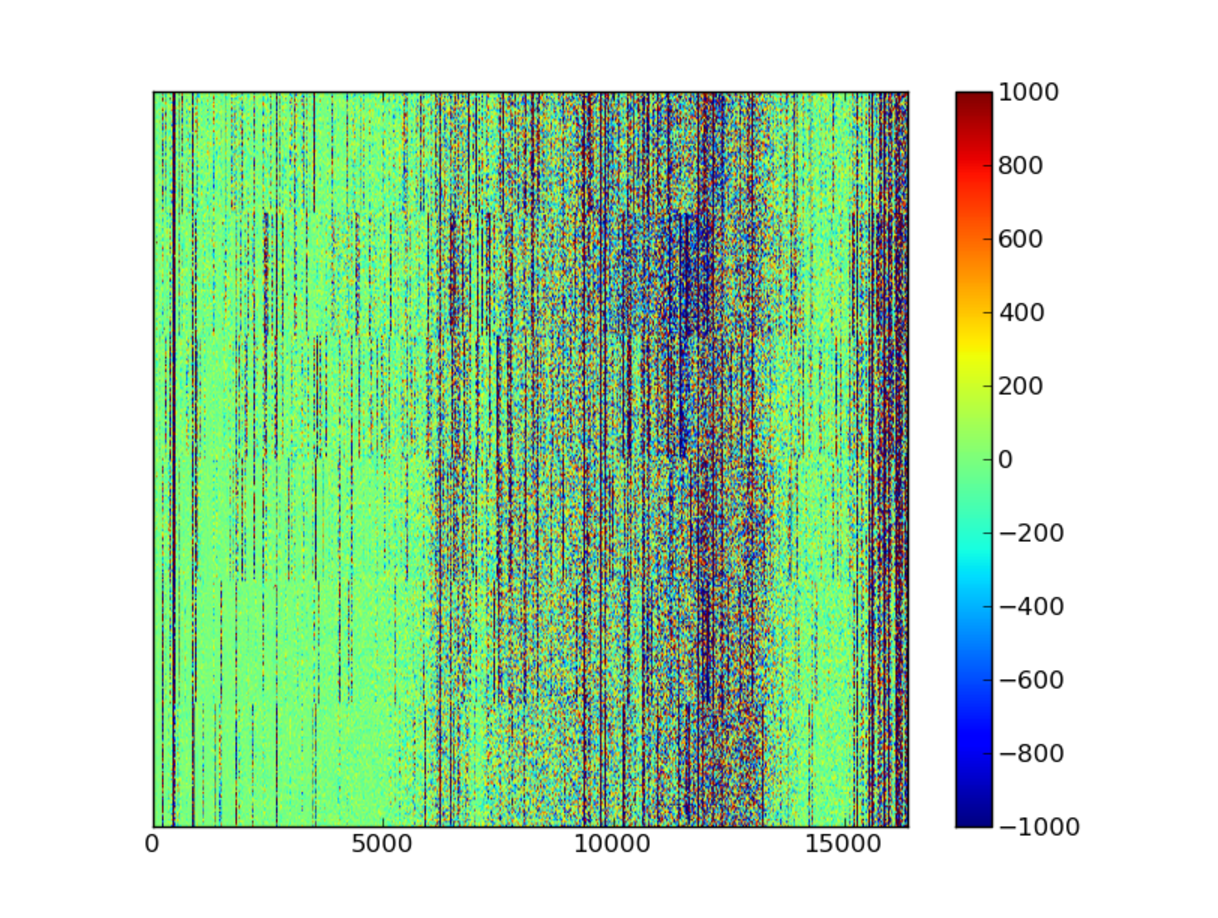
\includegraphics[width=1.3\linewidth]{1810fig1node9.pdf}
  \label{fig:sub1810node9}
\end{subfigure}%
\begin{subfigure}{0.5\textwidth}
  \centering
  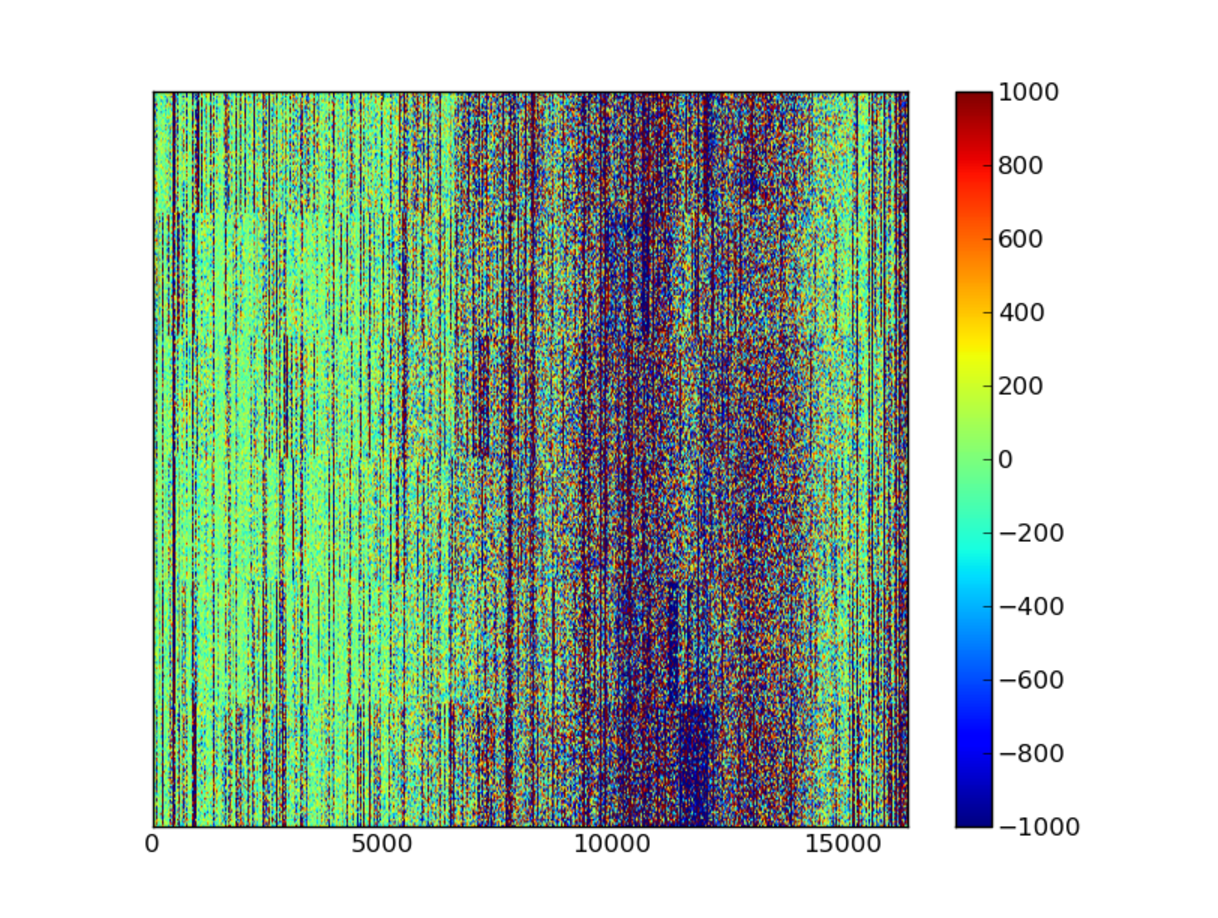
\includegraphics[width=1.3\linewidth]{1810fig2node7.pdf}
  \label{fig:sub1810node7}
\end{subfigure}
\caption{Plots of both polarizations of the millisecond pulsar J1810+1744 folded over an hour and a half with 16384 freqency channels and divded into 6 time bins along the y-axis. The x-axis is the number of the frequency bin, the colourbar the intesity of the signal.The left plot is the polarization recorded onto node9, the right is the polarization recorded onto node7. In neither is the pulsar visible.}
\label{fig:folding1810}
\end{figure}

\begin{figure}
\centering
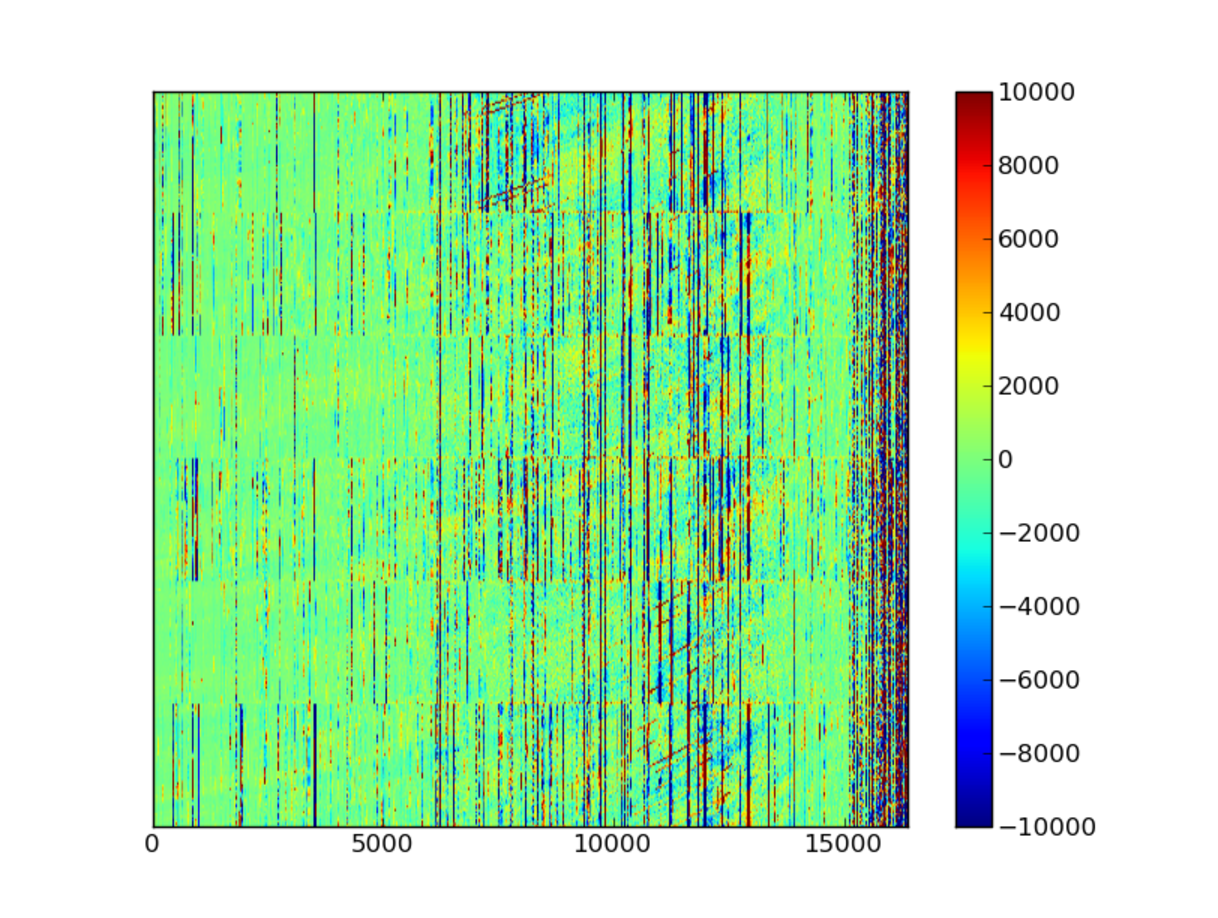
\includegraphics[width=\linewidth]{1919fig1node9.pdf}
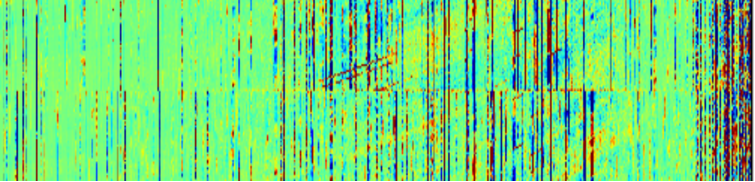
\includegraphics[width=\linewidth]{1919fig1node9crop.pdf}
\label{fig:folding1919}
\caption{Plots of both polarizations of the pulsar B1919+21 folded over 16 minutes with 16384 freqency channels and divded into 6 time bins along the y-axis. The x-axis is the number of the frequency bin, the colourbar the intesity of the signal. The plot shows the polarization recorded to node9. The pulsar is visible as a horizontal line. In this plot, it falls along the division between bins. The cropped portion below is a selection from the first two bins, the pulsar signal following the divide between them.}
\end{figure}

 
\end{document}
